\chapter{A Study on Common Vulnerabilities}
\label{chap:datasource}

In this chapter, present some strategies to select different \glspl{os} to be part of \gls{bft} replicated system.
These strategies are build from the data that is available on the vulnerability database developed in a previous work.
The promising results confirm the intuition that applying diversity implies vulnerability independence to some extent.
The contribution should make clear what are the security gains from using different \glspl{os} on a replicated intrusion-tolerant system.

\section{Methodology}

This section presents the methodology adopted in this study, with a particular focus on how the dataset was selected, processed, and analyzed.

%\subsection{Object of the study}

\subsection{Data Source}
We have analyzed \gls{os} vulnerability data from the \gls{nvd} database~\cite{nvd}. 
According to \gls{nist} a vulnerability is defined as follows:
%\gls{nvd} uses the \gls{cve} definition of vulnerability \cite{cveterm}, which is given below:

\begin{defn}
 \emph{``[...] A weakness in an information system, system security procedures, internal controls, or implementation that could be exploited by a threat source.''}~\cite{Nist:2012}
\end{defn}


%\gls{nvd} aggregates vulnerability reports from more than 70 security companies, forums, advisory groups and organizations,\footnote{See the complete list on \url{http://cve.mitre.org/compatible/alerts_announcements.html}.} being thus the most complete vulnerability database on the web.
%All data is made available as \gls{xml} files containing the reported vulnerabilities on a given period, called \emph{data feeds}.

\gls{nist}'s \gls{nvd} is the authoritative data source for disclosure of vulnerabilities and associated information. 
\gls{nvd} aggregates vulnerability reports from more than 70 security companies, advisory groups, and organizations, thus being the most extensive vulnerability database on the web. 
All data is made available as \gls{xml} data feeds, containing the reported vulnerabilities on a given period. 
Each \gls{nvd} vulnerability receives a unique identifier, in the format CVE-\textit{YEAR}-\textit{NUMBER}, and a short description provided by the \gls{cve}~\cite{cveterm}. 
The \gls{cpe}~\cite{cpe} provides the list of products affected by the vulnerability and the date of the vulnerability publication.
Additionally, the \gls{cvss}~\cite{cvss} calculates the vulnerability severity considering several attributes, such as the attack vector, privileges required, exploitability score, and the security properties compromised by the vulnerability (i.e., integrity, confidentiality, or availability).


We developed a program that collects, parses and inserts the \gls{xml} data feeds into an \gls{sql} database, deployed with a custom schema to group vulnerabilities by affected products and versions.

\paragraph{Chosen Products.}
In this thesis, we are mostly interested in \gls{ots} components. 
Contrary to automatic diversity mechanisms that need testing to assess the vulnerability correlation, \gls{ots} diversity can be supported by data evidence to understand the correlation between vulnerabilities and products. 
In particular, we focus on the diversity of \glspl{os} (not only the kernel but the whole product) for three fundamental reasons: (1) by far, most of the replica’s code is the \gls{os}; (2) such size and importance, make \glspl{os} a valuable target, with new vulnerabilities and exploits being discovered every day; and (3) there are many options of \glspl{os} that can be used.



\subsection{Data Selection}
Despite the vast amount of information about each vulnerability available in \gls{nvd}, for this study, we are only interested in the name, publication date, summary (description), type of exploit (local or remote), and list of affected products.
We have collected vulnerabilities reported for 64 \gls{cpe}~\cite{cpe}.
Each one of these describes a system, i.e., a stack of software/hardware components in which the vulnerability may be exploited.
These \gls{cpe} were filtered, resulting in the following information that was stored in our database:

\begin{itemize}
\item \textbf{Part:} \gls{nvd} separates this in Hardware, \gls{os} and Application. For the purpose of this study we choose only enumerations marked as \gls{os};
\item \textbf{Product:} The product name of the platform;
\item \textbf{Vendor:} Name of the supplier or vendor of the product platform.
\end{itemize}

In our previous work~\cite{Garcia:2012} we manually analysed those 64 \gls{cpe} and grouped them in 11 \gls{os} distributions: \textit{OpenBSD, NetBSD, FreeBSD, OpenSolaris, Solaris, Debian, Ubuntu, RedHat,\footnote{\textit{RedHat} comprises the ``old'' RedHat Linux (discontinued in 2003) and the newer RedHat Enterprise Linux (RHEL).} Windows2000, Windows2003} and \textit{Windows2008}.
These distributions cover the most used \emph{\gls{os} products} of the BSD, Solaris, Linux and Windows families.



%We did not include Mac~OS~X because, unlike for the included OSes, we did not have an OS~X system available for cross-validation of vulnerability reports.

%\begin{figure}[!ht]
% \centering
% \includegraphics[width=0.9\columnwidth]{images/ea-crop.pdf}
% \caption{Simplified SQL schema of the database used to store and analyze the \gls{nvd} data. Fields not displayed are only used for auxiliary purposes.}
% \label{ea}
%\end{figure}

%The schema of the resulting database is displayed in Figure \ref{ea}.
%The tables with prefix \textit{cvss}, \textit{vulnerability\_type} and \textit{security\_protection} are employed to optimize the database.
%The most important tables are:

%\begin{itemize}
%\item \emph{cvss\_*} tables: refer directly to the Common Vulnerability Scoring System (CVSS) metrics \cite{cvss} of the stored vulnerabilities, which quantify the severity and impact of vulnerabilities;
%\item \emph{vulnerability}: stores basic data about a vulnerability (name, publication date, etc.) from the \gls{nvd} augmented with vulnerability life cycle information from the Open Source Vulnerability Database (OSVDB) \cite{osvdb};
%\item \emph{vulnerability\_type}: stores the vulnerability type assigned by us (see Section \ref{vulntypes});
%\item \emph{os}: stores the \glspl{os} platforms of interest in this study;
%\item \emph{os\_vuln}: stores the relationship between vulnerabilities and \glspl{os}, and their affected versions.
%\end{itemize}

The use of an \gls{sql} database brought us at least three benefits when compared with analyzing the data directly from the \gls{xml} feeds.
First, it allows us to \emph{enrich the data set} by hand, for example, by associating release times and family names to each affected \gls{os} distribution.
Second, it allows us to modify the \gls{cve} fields to correct problems.
For instance, one of the problems with \gls{nvd} is that the same product is occasionally registered with distinct names in different entries;
For instance, (\textit{debian\_linux}, \textit{debian}) and (\textit{linux}, \textit{debian}) are two (product, vendor) pairs we have found for the Debian Linux distribution.
Other users of \gls{nvd} data feeds previously observed this same problem~\cite{cvedetails}.
Finally, an \gls{sql} database is much more convenient to work with than parsing the feeds on demand.

\subsection{Filtering the Data}\label{filtering_data}
The following steps were taken during the work~\cite{Garcia:2012} prior to this thesis, however, for the extended contributions we had to re-do some of the steps to keep the database updated.
From both works, we selected a  selected 2563 vulnerabilities from a total of more than 44,000 vulnerabilities published by \gls{nvd}.
These vulnerabilities are the ones classified as \gls{os}-level vulnerabilities (``/o'' in their \gls{cpe}) for the \glspl{os} under consideration.

When manually inspecting the data set, we discovered and removed vulnerabilities that contained tags in their descriptions such as \emph{Unknown} and \emph{Unspecified}. 
These correspond to vulnerabilities for which \gls{nvd} does not know precisely where they occur or why they exist (however, they are usually included in the \gls{nvd} database because they were mentioned in some patch released by a vendor). 
We also found few vulnerabilities flagged as \emph{**DISPUTED**}, meaning that product vendors disagree that the vulnerability exists, and \emph{Duplicate}, used for vulnerabilities in which the \emph{summary} points to a duplicate entry or duplicate entry suspicion.
Due to the uncertainty that surrounds these vulnerabilities, we decided to exclude them from the study as well.

Table \ref{tab:unknowns} shows the distribution of these vulnerabilities across the analyzed \glspl{os}, together with the total number of valid vulnerabilities.

%TABLE 1
\begin{table}[!ht]
\begin{center}
{\scriptsize
\begin{tabular}{|l||c | c | c | c | c|}\hline
\textbf{OS} & \textbf{Valid} & \textbf{Unknown} & \textbf{Unspecified} & \textbf{Disputed} & \textbf{Duplicate}  \\\hline\hline % total
OpenBSD & 153 & 1 & 1 & 1 & 0 \\
NetBSD & 143 & 0 & 1 & 2 & 0  \\
FreeBSD & 279 & 0 & 0 & 2 & 0 \\
OpenSolaris & 31 & 0 & 52 & 0 & 0  \\
Solaris & 426 & 40 & 145 & 0 & 3  \\
Debian & 213 & 3 & 1 & 0 & 0  \\
Ubuntu & 90 & 2 & 1 & 0 & 0  \\
RedHat & 444 & 13 & 8 & 1 & 1  \\
Windows2000 & 495 & 7 & 28 & 5 & 5  \\
Windows2003 & 56 & 5 & 34 & 3 & 5  \\
Windows2008 & 334 & 0 & 8 & 0 & 3   \\\hline\hline
\textbf{\#distinct vulns.} & 2270 & 63 & 210 & 8 & 12 \\ \hline
\end{tabular}
\caption{Distribution of OS vulnerabilities in NVD.}
\label{tab:unknowns}
}
\end{center}
\end{table}

An important observation about Table \ref{tab:unknowns} is that the columns do not add up to the number of distinct vulnerabilities (last row of the table) because some vulnerabilities are shared among \glspl{os} and are counted only once.
Notice that about 60\% of the removed vulnerabilities affected Solaris and OpenSolaris.
Moreover, these two systems are the only ones that have more than 10\% of its vulnerabilities removed.
We should remark that this manual filtering was necessary to increase the confidence that only valid vulnerabilities were used in the study.


\section{OS Diversity Study}\label{study}
This section analyzes the vulnerabilities that were shared in \gls{os} pairs over the period of 1994 to 2011. 
In the investigation, we consider two possible server machine setups offering an increasingly more secure platform. 
This accommodates the case where system administrators create differentiated \gls{os} installations, which contain more or less vulnerabilities depending on the services and applications available in the server. 
Of course, other setups could be used, but we decided to concentrate on these configurations because they are quite generic and they lead to results that can be directly obtained from the \gls{nvd} data. 
The setups are the following:

\begin{itemize}

\item \textbf{Fat Server:} The server contains most of the software packages for a given \gls{os}, and consequently, it can be used to run various kinds of applications by locally or remotely connected users. This server has potentially all vulnerabilities that were reported for the corresponding \gls{os};

%\item \textbf{Thin Server:} This setting corresponds to a platform that does not contain any applications (except for the replicated service). The server has a decreased security risk because the attack vectors related to applications have been mostly eliminated. 
%In this setting, vulnerabilities classified as \textit{Applications} are excluded from the statistics;

\item \textbf{Isolated Thin Server:} This setting corresponds to a platform that does not contain any applications (except for the replicated service). 
The server has a decreased security risk because the attack vectors related to applications have been mostly eliminated. 
Moreover, is placed in a room physically protected from illegal accesses, with remote logins disabled, and therefore it can only be compromised by receiving malicious packets from the network. In this setting, we only consider remotely exploitable vulnerabilities (those with ``Network'' or ``Adjacent Network'' values in their CVSS\_ACCESS\_VECTOR field) that are not classified as \textit{Applications}.

\end{itemize}

The Fat Server setup corresponds to a case where an attack may target an application available in the \gls{os} distribution. 
Therefore, it provides an upper bound estimate on the number of vulnerabilities that can be exploited. 
The Isolated Thin Server setup is the counterpart case, where the system is deployed without applications that come bundled with the \gls{os} and thus provide a lower bound estimate on the number of common vulnerabilities and it has the vulnerabilities that can be remotely exploited. 
Of course, in practice, at least one application (such as a name service or a distributed file service) would be deployed in an intrusion-tolerant system, and the vulnerabilities of this application would add up to the flaws that we will report. 
In any case, since we expect that most of the complexity is in the \gls{os}, we anticipate that a single application will have a small contribution to the overall number of vulnerabilities.



Intrusion-tolerant systems are usually built using four or more replicated servers~\cite{Castro:2002}. 
Therefore, it is useful to understand if there are many vulnerabilities that involve groups of \glspl{os} larger than two -- if this is the case, then it will be hard to find \gls{os} configurations for the various servers that do not share vulnerabilities, and a goal of using \gls{ots} diversity will be difficult to be achieved in practice. 
Figure \ref{top} portrays the number of common vulnerabilities that exist simultaneously in increasingly more extensive sets of \glspl{os} (with Isolated Thin Servers). 
The graph shows a rapid decrease in the shared vulnerabilities as the number of \glspl{os} grows. 
The largest group that was affected by the same vulnerability had six \glspl{os}, and this occurred only for a single flaw, and there were also two vulnerabilities in sets with five \glspl{os}. Vulnerabilities in two and three \glspl{os} usually occur in systems from the same family, whose common ancestry implies the reuse of more significant portions of the code base.
%As we have seen in previous tables, this is particularly true for the Windows and BSD families.

\begin{figure}[!h]
 \centering
 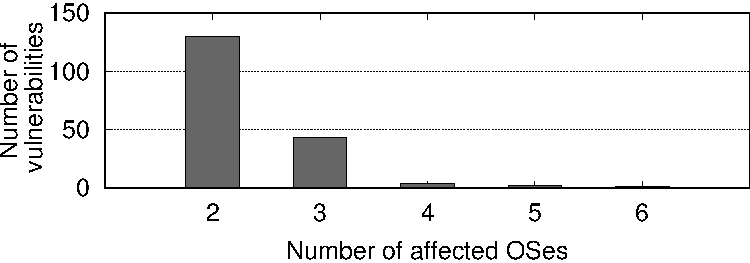
\includegraphics[]{images/gnuplot/spe/top/top.pdf}
 \caption{Common vulnerabilities for $n$ different OSes (with Isolated Thin Servers).}
 \label{top}
\end{figure}


Table \ref{tab:spreaded_vulns} lists in more detail the vulnerabilities that can be exploited in larger groups (four to six) of \glspl{os}. 
The first three bugs have a considerable impact because they allow a remote adversary to run arbitrary commands on the local system using a high-privilege account. 
They occurred either in widespread login services (telnet and rlogin) or in a primary system function, and consequently, several products from the BSD family were affected, as well as Solaris. 
The \gls{nvd} entry for the CVE-2001-0554 vulnerability also had external references to the Debian and RedHat websites, which could indicate that these systems might suffer from a similar (or the same) problem. 
Vulnerability CVE-2008-1447 occurs in a large number of systems because it results from a bug in the BIND implementation of the \gls{dns}. Since BIND is a highly popular service, more \glspl{os} could potentially be affected. 
A closer look at the corresponding \gls{nvd} entry reveals external references to the sites of OpenBSD, NetBSD, and FreeBSD, indicating that they would be vulnerable in case this software was being used. 
This sort of vulnerability confirms that from an intrusion-tolerance perspective it is unwise to run the same server software everywhere, and that diverse implementations must be selected (in this case for recursive \gls{dns} servers).


\begin{table}[!ht]
\begin{center}
{\scriptsize
\begin{tabular}{|c||c| p{7,8cm} | }\hline
\textbf{CVE} & \#affected OS  & Description  \\\hline\hline
CVE-1999-0046  &  4  & Buffer Overflow of \emph{rlogin} allows admin access. Affects: NetBSD, FreeBSD, Solaris and Debian. \\ \hline
CVE-2001-0554  &  4  & Buffer overflow in telnetd (telnet daemon) allows remote attackers to execute arbitrary commands. Affects: OpenBSD, NetBSD, FreeBSD and Solaris.  \\ \hline
CVE-2003-0466  &  4  & Off-by-one error in the Kernel function \emph{fb\_realpath()} allows admin access. Affects: OpenBSD, NetBSD, FreeBSD and Solaris.  \\ \hline
CVE-2005-0356  &  4  & TCP implementations allow a denial of service (DoS) via spoofed packets with large timer values, when used with Protection Against Wrapped Sequence Numbers. Affects: OpenBSD, FreeBSD, Windows2000 and Windows2003. \\ \hline
CVE-2008-1447  &  5  & The BIND 8 and 9 implementation of the DNS protocol allow attackers to spoof DNS traffic via a birthday attack to conduct cache poisoning against recursive resolvers. Affects: Debian, Ubuntu, RedHat, Windows2000 and Windows2003.  \\ \hline
CVE-2001-1244  &  5  & TCP implementations allow a DoS by setting a maximum segment size very small to force the generation of more packets, amplifying network traffic and CPU consumption. Affects: OpenBSD, NetBSD, FreeBSD, Solaris and Windows2000. \\ \hline
CVE-2008-4609  &  6  & TCP implementation allows a DoS via multiple vectors that manipulate TCP state table. Affects: OpenBSD, NetBSD, FreeBSD, Windows2000, Windows2003 and Windows2008.   \\ \hline
\end{tabular}
}
\caption{Vulnerabilities that affect more than four OSes.}
\label{tab:spreaded_vulns}
\end{center}
\end{table}


The remaining three vulnerabilities are related to the protocol stack of \gls{tcp}/\gls{ip}. 
All of them affect system availability, allowing different forms of \gls{dos} attacks. 
CVE-2008-4609 is the vulnerability that affects more \glspl{os}, according to the \gls{nvd} database, because \gls{tcp}/\gls{ip} stack code is often reused across \glspl{os}.%, we checked the websites of the other \glspl{os} for reports related to this vulnerability. 
%We only found a disclaimer by RedHat~\footnote{\url{https://access.redhat.com/kb/docs/DOC-18730}} stating that this flaw affected some releases but that they would not provide an update (they only offered a mitigation solution based on IPtables, the Linux firewall software).

Overall, the above results look encouraging because over a significant period (around 18 years) there are very few vulnerabilities that appear in many \glspl{os}. 
A good portion of them are in the \gls{tcp}/\gls{ip} stack implementation, which is probably the most shared software component across \glspl{os}, but they only impact on the availability of the system, leaving confidentiality and integrity of data unharmed.


\section{Strategies for OS Diversity Selection}\label{sec:datasource_evaluation}
The preliminary analysis indicates that it is possible to find that some \glspl{os} share fewer vulnerabilities than others. 
Therefore, in this section we present three alternative strategies to select \glspl{os}, based on the built dataset, to decrease the chance of common vulnerabilities on replicated systems. 
We start the section by first describing an approach we called the \gls{cvi}, which is used by one of the strategies. 
For each strategy, we then give example sets of \glspl{os} that exhibit a reasonable level of diversity, and perform an evaluation based on the collected data. 
Finally, we conclude the section with an analysis of potential diversity between releases of the same \glspl{os} (concentrating on the \glspl{os} that the three strategies picked as the best configuration).


\subsection{Common Vulnerability Indicator}\label{cvi}
In our previous work~\cite{Garcia:2012} we have found that the number of common vulnerabilities that are observed between different \glspl{os} varies over time. 
Thus, in order to be able to evaluate which \gls{os} pairs are more (or less) likely to experience common flaws while taking into account the timing of vulnerability disclosures, we developed a new metric, called the \emph{\gls{cvi}}. 
This indicator is calculated for a given year $y$, based on the vulnerabilities that were shared by \glspl{os} A and B over a period of $\mathit{tspan}$ previous years. \gls{cvi} is built to ensure the following desirable properties:
\begin{enumerate}
\newcommand{\OLDtheenumi}{\theenumi}
\renewcommand{\theenumi}{\roman{enumi}}
\item $\mathit{CVI}_y(A,B) = 0$ if A and B have no common vulnerabilities in the $\mathit{tspan}$ interval;
\item $\mathit{CVI}_y(A,B) < \mathit{CVI}_y(C,D)$ if A and B shared less vulnerabilities than C and D in each year of the considered period;
\item $\mathit{CVI}_y(A,B) < \mathit{CVI}_y(C,D)$ if A and B had $N$ common vulnerabilities in the distant past while C and D had $N$ shared vulnerabilities more recently;
\item $\mathit{CVI}_{y_2}(A,B) < \mathit{CVI}_{y_1}(A,B)$, with $y_1 < y_2$, if the number of common vulnerabilities for A and B has decreased over the years.
\renewcommand{\theenumi}{\OLDtheenumi}
\end{enumerate}

Therefore, \gls{cvi} is useful for comparison purposes, allowing the identification of \gls{os} pairs that have a smaller number of common flaws, while considering the instant when vulnerabilities were found. 
This last point is particularly crucial because \glspl{os} are continually evolving, potentially getting more (or less) diverse, and consequently, one should take into consideration the time dimension when selecting \gls{os} configurations (e.g., \gls{os} pairs that have had less common flaws recently are likely better candidates).
\gls{cvi} is computed as follows:

First, a weighting factor $\alpha_{i}$ is defined for each year   $i \in \{y-\mathit{tspan}+1, ..., y-2, y-1, y\}$.

\begin{equation}
\alpha_{i} = 1 - \frac{y-i}{\mathit{tspan}}
\end{equation}

Then, CVI is obtained using the number of vulnerabilities $v_{i}(A,B)$ that appeared in both \glspl{os} A and B for every year $i$ from the start of the time span up to reference year $y$.

\begin{equation}
\mathit{CVI}_{y}(A,B)= \sum_{i = y-\mathit{tspan}+1}^{y} \alpha_{i}\cdot v_{i}(A,B)
\end{equation}


\begin{table}[!ht]
\begin{center}
{\scriptsize
\begin{tabular}{|l|c c c|| c c c |}
\cline{2-7}
\multicolumn{1}{c}{} &  \multicolumn{3}{|c||}{\textbf{Fat Server}}  &  \multicolumn{3}{|c|}{\textbf{Isolated Thin Server}} \\ \hline
OS             & 2009 &	2010 & 	2011        & 	2009 & 	2010 & 2011 \\ \hline
OpenBSD-NetBSD  & 17.1 & 13.8 & 14.8        & 8.4 & 7.1 & 6.9   \\
OpenBSD-FreeBSD & 22.2 & 18.0 & 18.1        & 14.1  & 11.6 & 10.3  \\
OpenBSD-Solaris & 4.0 & 3.1 & 3.3           &  1.8 & 1.4 & 0.9  \\
OpenBSD-Debian
  & 1.7 & 1.5 & 1.4           &  0.0 & 0.0 & 0.0  \\
OpenBSD-RedHat & 5.0 & 4.1 & 3.2           &  1.6 & 1.4 & 1.1  \\
OpenBSD-Win2000 & 1.8 & 1.5 & -             &  1.8 & 1.5 & -  \\  \hline
NetBSD-FreeBSD  & 19.7 & 18.3 & 18.8        & 11.0 & 9.3 & 8.6 \\
NetBSD-Solaris  & 4.9 & 4.0 & 4.2           &  1.5 & 1.1 & 0.7  \\
NetBSD-Debian   & 1.4 & 0.9 & 0.5           &  0.6 & 0.4 & 0.2  \\
NetBSD-RedHat  & 1.8 & 1.1 & 0.5           &  0.6 & 0.4 & 0.2  \\
NetBSD-Win2000  & 1.6 & 1.4 & -             & 1.6 & 1.4 & -   \\ \hline
FreeBSD-Solaris & 6.5 & 5.4 & 6.3           & 2.3 & 1.7 & 1.2  \\
FreeBSD-Debian  & 1.3 & 0.8 & 0.5           & 0.0 & 0.0 & 0.0  \\
FreeBSD-RedHat & 5.6 & 4.4 & 3.3           & 1.7 & 1.4 & 1.1  \\
FreeBSD-Win2000 & 2.3 & 1.9 & -             & 2.3 & 1.9 & -  \\ \hline
Solaris-Debian  & 1.0 & 0.8 & 0.6           & 0.0 & 0.0 & 0.0  \\
Solaris-RedHat & 5.3 & 6.5 & 5.5           & 1.0 & 0.7 & 0.5  \\
Solaris-Win2000 & 5.5 & 5.7 & -             & 1.0 & 0.7 & -  \\ \hline
Debian-RedHat  & 26.1 & 20.5 & 15.7        & 3.2 & 2.1 & 1.4  \\
Debian-Win2000  & 0.9 & 0.8 & -             & 0.9 & 0.8 & -   \\ \hline
RedHat-Win2000 & 1.8 & 1.6 & -             & 0.9 & 0.8 & -   \\ \hline
\end{tabular}
\caption{CVI for the years 2009 to 2011, with $\mathit{tspan}$ of 10 years.}
\label{tab:cvi-2011-2009}
}
\end{center}
\end{table}

Table~\ref{tab:cvi-2011-2009} presents \gls{cvi} values for the years 2009 to 2011. 
We have excluded from this analysis \glspl{os} with vulnerability information missing for more than one year over the period, to avoid using incomplete data in the calculation of the indicators. Therefore, the following \glspl{os} were not considered in Table~\ref{tab:cvi-2011-2009}: Windows2003, Windows2008, Ubuntu, and OpenSolaris. 
The \gls{cvi} values are computed for a $\mathit{tspan}$ of 10 years to reflect a reasonable history. 
It is possible to see that, except for one system (Solaris with FreeBSD/RedHat/Windows2000 in the Fat Server), in all remaining cases \gls{cvi} shows a decreasing trend. 
Several of the \glspl{os} that have evolved over a considerable period are having less reported vulnerabilities, and this causes a decline in shared vulnerabilities in recent years. 
For some of the \gls{os} pairs the drop in the \gls{cvi} value is quite significant, becoming almost one-third of the 2009 value (NetBSD with Debian or RedHat). 
In the Isolated Thin Server case, there are three pairs with $\mathit{CVI}(A,B)=0$, which shows that they have shared no vulnerabilities during the past 12 years, and are thus particularly good candidates to include in intrusion-tolerant configurations. 
These systems are Debian with either OpenBSD or FreeBSD or Solaris.

%According to Table~\ref{tab:pairs_vulns_by_year}, both \gls{os} pairs had 10 common vulnerabilities in the 2000--2011 period, suggesting that they both provide the same degree of diversity. 
From the \gls{cvi} values in Table~\ref{tab:cvi-2011-2009}, it is apparent that OpenBSD and RedHat have become more diverse, in recent years, than RedHat and Solaris, and to make it advisable, from a diversity standpoint, to choose the former \gls{os} pair over the latter.



\subsection{Building Replicated Systems with Diversity}
\label{build_diversity}


This section describes three strategies for choosing diverse sets of \glspl{os}. 
These strategies utilize the data analyzed earlier as a basis to make decisions, by assuming that the information reported by \gls{nvd} on vulnerabilities can be correlated to the amount of diversity among \glspl{os}. 
Of course, there are some caveats associated with this approach, but the alternatives can be even harder to put in practice, especially if one wants to consider a large number of \glspl{os}. 
For example, for closed systems (e.g., Windows) it is challenging to determine the level of sharing of \gls{os} components, and therefore, diversity estimations based on the code cannot be performed. Moreover, even if this estimate could be obtained, there is the risk that it does not reflect the number of vulnerabilities that occur simultaneously in several \glspl{os} (e.g., two distinct implementations of the same flawed algorithm are vulnerable).

The first strategy, called \gls{cvcs}, is based on raw data collected over a considerable interval, and it is the most straightforward approach for selecting \gls{os} pairs.
It should be used when one wants to treat all vulnerabilities, regardless of the time which they were reported, as equally important to make choices. 
The second strategy, \gls{cvis}, uses the \gls{cvi} described in the previous section to select \gls{os} pairs taking into account the incidence of common vulnerabilities over the years. 
It is indicated when one wants to give greater importance to more recent vulnerabilities because it is a weighted sum. 
The third strategy, \gls{irts}, follows a different approach from the previous ones, focusing not so much on common vulnerabilities directly, but on the frequency in which vulnerabilities appear in the two \glspl{os}. 
If one wants to give more importance to the time interval between successive reports of common vulnerabilities, this is the best strategy. 
Since this last criterion complements the previous two, one could explore strategies \gls{cvcs} and \gls{cvis} in conjunction with \gls{irts}.

For every strategy, we present \gls{os} sets examples for the Fat Server and Isolated Thin Server configurations. 
Fat Server configurations can be pessimistic in the sense that they may account for common vulnerabilities in applications that are not present in the servers, while Isolated Thin Server configurations reflect more accurately the expected setup of dedicated servers in a replicated system. 
An intrusion-tolerant system usually requires $3f+1$ replicas to tolerate $f$ intrusions (e.g., \cite{Castro:2002}). 
Therefore, we will focus on sets with four \glspl{os} to deploy a hypothetical replicated system with four replicas, which allows one fault to be tolerated.

As a cautious note, one should take into account that Ubuntu and Windows2008 were first released in 2004 and 2008 respectively, so the data for these two \glspl{os} was collected for a smaller number of years. 
Windows2000 is presented in the tables because there are published vulnerabilities until 2010, although it has been gradually replaced by Windows2003 and Windows2008 in the organizations. Consequently, we do not use Windows2000 when choosing the \gls{os} sets. 
We have excluded OpenSolaris from the study because there is data available for only a limited period. 
In each strategy and configuration, we present two sets: \emph{setCon} is more conservative, since it does not contain Ubuntu and Windows2008; and \emph{setUpdt} is more up-to-date because it can include Ubuntu and Windows2008. 
When looking at these two sets, one should keep in mind that setCon is selected from a group of \glspl{os} for which there is a significant amount of \gls{nvd} data, which contributes for higher confidence on the result. 
On the other hand, setUpdt uses \glspl{os} with different amounts of \gls{nvd} data, which can cause small levels of inaccuracy when making comparisons (e.g., in the \gls{cvcs}, any \gls{os} pair featuring Windows2008 has zero common vulnerabilities until 2007). 
One way to address this would be only to consider vulnerabilities that appear later than 2007 when choosing setUpdt. 
We opted not to follow this approach because it has the drawback of discarding too much data.


\subsection{Common Vulnerability Count (CVCst)} 

The results from the previous section give a strong indication that it should be possible to choose groups of \glspl{os} with a few common vulnerabilities over reasonable intervals of time. 
However, we would like to understand if the data from the \gls{nvd} database is effective at suggesting these groups of \glspl{os}. 
To address this point, we divided the data into two subsets: the \emph{history period}, comprising the data for the interval between 2000 to 2009, and the \emph{observed period}, from 2010 to 2011. 
The objective is to employ the historical period to pick the sets of \glspl{os} to use on the replicated system (as if the choice was made at the beginning of 2010). Then we use the data for the observed period to verify if these choices would have been adequate, i.e., if they have a small (preferably the smallest) number of common vulnerabilities in this period.

\gls{cvcs} makes decisions based directly on the empirical data for the number of common vulnerabilities across all \gls{os} pairs. 
This data is displayed in Table \ref{tab:strat_i} for \glspl{os} with a Fat Server configuration. 
Numbers to the right and above the diagonal line represent the history period, while numbers to the left and below the line stand for the observed period. 
For example, the entry corresponding to OpenBSD-RedHat to the right of the diagonal line has the number 10, which means that these \glspl{os} shared 10 vulnerabilities between 2000 and 2009. 
The equivalent entry, but to the left of the diagonal line, is 0 because they had no common flaws reported in 2010 and 2011. 
As expected, \gls{os} pairs from the same family had the highest counts of common vulnerabilities. 
The only case where there were more vulnerabilities in the observed period than the historical period is for the Windows2008--Windows2003 pair, which is explained by the recent release date of Windows2008. 
It is interesting to notice, however, that most pairs had zero common vulnerabilities in the observed period.


\begin{table}[!ht]
\begin{center}
{\footnotesize
\begin{tabular}{|l|c|c|c|c|c|c|c|c|c|c|c|c|}\cline{2-11}
 \multicolumn{1}{c|}{} &
\begin{sideways}\vspace{2mm}\parbox{2mm}OpenBSD\end{sideways}&
\begin{sideways}\vspace{2mm}\parbox{2mm}NetBSD\end{sideways}&
\begin{sideways}\vspace{2mm}\parbox{2mm}FreeBSD\end{sideways}&
\begin{sideways}\vspace{2mm}\parbox{2mm}Solaris  \end{sideways}&
\begin{sideways}\vspace{2mm}\parbox{2mm}Debian\end{sideways}&
\begin{sideways}\vspace{2mm}\parbox{2mm}Ubuntu \end{sideways}&
\begin{sideways}\vspace{2mm}\parbox{2mm}RedHat\end{sideways}&
\begin{sideways}\vspace{2mm}\parbox{3mm}Win2000 \end{sideways}&
\begin{sideways}\vspace{2mm}\parbox{3mm}Win2003 \end{sideways}&
\begin{sideways}\vspace{2mm}\parbox{3mm}Win2008  \end{sideways}&
\multicolumn{2}{|c}{} \\ \cline{1-11}  \cline{1-12}
OpenBSD & - & 33 & 43 & 9 & 2 & 3 & 10 & 3 & 2 & 1&   \multirow{13}{1mm}{\begin{sideways}\hspace{8mm}\parbox{15mm}{2000-2009}\end{sideways}} \\ \cline{1-11}
NetBSD & 4 & - & 36 & 9 & 4 & 0 & 6 & 3 & 2 & 1  &\\ \cline{1-11}
FreeBSD & 4 & 6 & - & 12 & 4 & 2 & 12 & 4 & 3 & 1& \\ \cline{1-11}
Solaris & 1 & 1 & 2 & - & 2 & 2 & 8 & 8 & 7 & 0 &\\ \cline{1-11}
Debian & 0 & 0 & 0 & 0 & - & 14 & 52 & 1 & 1 & 0 &\\ \cline{1-11}
Ubuntu & 0 & 0 & 0 & 0 & 0 & - & 27 & 1 & 1 & 0 &\\ \cline{1-11}
RedHat & 0 & 0 & 0 & 2 & 0 & 0 & - & 2 & 2 & 0 &\\ \cline{1-11}
Win2000 & 0 & 0 & 0 & 1 & 0 & 0 & 0 & - & 216 & 42 &\\ \cline{1-11}
Win2003 & 0 & 0 & 0 & 1 & 0 & 0 & 0 & 49 & - & 53 & \\ \cline{1-12}
Win2008 & 0 & 0 & 0 & 1 & 0 & 0 & 0 & 38 & 229 & -	& \multicolumn{1}{|c}{}  \\ \cline{1-11}
 \multicolumn{1}{c|}{}& \multicolumn{9}{|c|}{2010-2011} & \multicolumn{2}{|c}{}\\ \cline{2-10}
\end{tabular}
\caption{History/observed period for CVCst with Fat Servers.}
\label{tab:strat_i}
}
\end{center}
\end{table}


The strategy for building sets of \glspl{os} is based on a simple cost function. 
Given any potential \gls{os} pair A and B that could be added to the set, one can perform a lookup in Table \ref{tab:strat_i} to determine the pair's number of common vulnerabilities in the historical period. 
This number corresponds to the cost of adding this \gls{os} pair to the group. 
Similarly, when including a third \gls{os} C, it is possible to find in the table the entries for A--C and B--C and take their sum as the cost of integrating C in the group. 
When building a set with $n$ \glspl{os}, the total cost is the addition of each individual cost for all combinations of \gls{os} pairs.
The sets that lead to smaller values of total cost are considered the best choices for deployment in the replicated system.
Accordingly, based on the table, the best groups of four \glspl{os} are:

\begin{itemize}
  \setlength\itemsep{0em}
\item setCon = \{\emph{OpenBSD, Solaris, Debian, Windows2003}\}, with a total cost of 23;
\item setUpdt = \{\emph{NetBSD, Solaris, Ubuntu, Windows2008}\}, with a total cost of 12.%, but one vulnerability affects more than two \glspl{os} simultaneously, hence two pairs.
\end{itemize}


One, however, should keep in mind that sometimes the total cost may be only an approximation of the actual number of shared vulnerabilities among the \glspl{os} in the set, as specific vulnerabilities might be counted more than once. 
This will likely not be a problem since overcounting vulnerabilities provides a conservative estimate, or an estimate worse than reality. 
For example, setUpdt only has 11 shared vulnerabilities for a total cost of 12, since one of the vulnerabilities appears in three of the \glspl{os} (and is therefore included in two table entries).

Next we can check to what extent our choice of the best group of four \glspl{os} that we would pick from the historical period (2000--2009), as prescribed by \gls{cvc} cost calculation, remains consistent with the choice of the best group of four \glspl{os} from the observed period (2010--2011). 
We see that both setCon and setUpdt have only two shared vulnerabilities. 
They are not the best sets in the observed period (2010--2011), since there are groups of \glspl{os} with zero common vulnerabilities in the observed period (e.g., by replacing Solaris with RedHat), though they do exhibit a high level of diversity. 
A graphical representation of the sets as Venn diagrams is available in Figures~\ref{fig-venn_a}(a) and~\ref{fig-venn_a}(b). 
Below the \gls{os} name is the total number of vulnerabilities during the observed period, and the number inside each intersection shows the count of common flaws for the corresponding \glspl{os}. 
For example, in setCon with Fat Servers (Figure~\ref{fig-venn_a}(a)) there is one vulnerability that appears both on Solaris and OpenBSD and another on Solaris and Windows2003.


\begin{table}[!ht]
\begin{center}
{\footnotesize
\begin{tabular}{|l|c|c|c|c|c|c|c|c|c|c|c|c|}\cline{2-11}
 \multicolumn{1}{c|}{} &
\begin{sideways}\vspace{2mm}\parbox{2mm}OpenBSD\end{sideways}&
\begin{sideways}\vspace{2mm}\parbox{2mm}NetBSD\end{sideways}&
\begin{sideways}\vspace{2mm}\parbox{2mm}FreeBSD\end{sideways}&
\begin{sideways}\vspace{2mm}\parbox{2mm}Solaris  \end{sideways}&
\begin{sideways}\vspace{2mm}\parbox{2mm}Debian\end{sideways}&
\begin{sideways}\vspace{2mm}\parbox{2mm}Ubuntu \end{sideways}&
\begin{sideways}\vspace{2mm}\parbox{2mm}RedHat\end{sideways}&
\begin{sideways}\vspace{2mm}\parbox{3mm}Win2000 \end{sideways}&
\begin{sideways}\vspace{2mm}\parbox{3mm}Win2003 \end{sideways}&
\begin{sideways}\vspace{2mm}\parbox{3mm}Win2008  \end{sideways}&
\multicolumn{2}{|c}{} \\ \cline{1-11}  \cline{1-12}
OpenBSD & - & 13 & 26 & 5 & 0 & 0 & 3 & 3 & 3 & 1&\multirow{13}{1mm}{\begin{sideways}\hspace{8mm}\parbox{15mm}{2000-2009}\end{sideways}} \\ \cline{1-11}
NetBSD & 1 & - & 18 & 4 & 2 & 0 & 2 & 3 & 1 & 1& \\ \cline{1-11}
FreeBSD & 1 & 1 & - & 6 & 0 & 0 & 3 & 4 & 2 & 1& \\ \cline{1-11}
Solaris & 0 & 0 & 0 & - & 0 & 0 & 2 & 2 & 1 & 0& \\ \cline{1-11}
Debian & 0 & 0 & 0 & 0 & - & 2 & 8 & 1 & 1 & 0 &\\ \cline{1-11}
Ubuntu & 0 & 0 & 0 & 0 & 0 & - & 1 & 1 & 1 & 0 &\\ \cline{1-11}
RedHat & 0 & 0 & 0 & 0 & 0 & 0 & - & 1 & 1 & 0 &\\ \cline{1-11}
Win2000 & 0 & 0 & 0 & 0 & 0 & 0 & 0 & - & 81 & 13 &\\ \cline{1-11}
Win2003 & 0 & 0 & 0 & 0 & 0 & 0 & 0 & 4 & - & 14 &\\ \cline{1-12}
Win2008 & 0 & 0 & 0 & 0 & 0 & 0 & 0 & 3 & 26 & - & \multicolumn{1}{|c}{}  \\ \cline{1-11}
 \multicolumn{1}{c|}{}& \multicolumn{9}{|c|}{2010-2011} & \multicolumn{2}{|c}{}\\ \cline{2-10}
\end{tabular}
\caption{History/observed period for strategy CVCst with Isolated Thin Servers.}
\label{tab:strat_i_iso}
}
\end{center}
\end{table}


Table \ref{tab:strat_i_iso} presents the common vulnerabilities with the Isolated Thin Server configuration data. This configuration represents a class of servers that have a dedicated function and are protected against physical intruders. 
The same approach can be applied as above: first, we choose the best pairs based on the historical period to build a set of four \glspl{os}; next, we evaluate the sets by comparing the results with the values for the observed period. 
The history period provides two candidate sets: 

\begin{itemize}
\item setCon = \{\emph{NetBSD, Solaris, Debian, Windows2003}\}, with a total cost of 9;
\item setUpdt = \{\emph{Solaris, Debian, Ubuntu, Windows2008}\}, with a total cost of 2.
\end{itemize}

In the observed period, setCon and setUpdt have no common vulnerabilities, showing that the strategy would have chosen sufficiently diverse groups of \glspl{os}. A graphical representation of the sets is displayed in Figures~\ref{fig-venn_a}(c) and~\ref{fig-venn_a}(d).

\begin{figure}[!h]
 \centering
 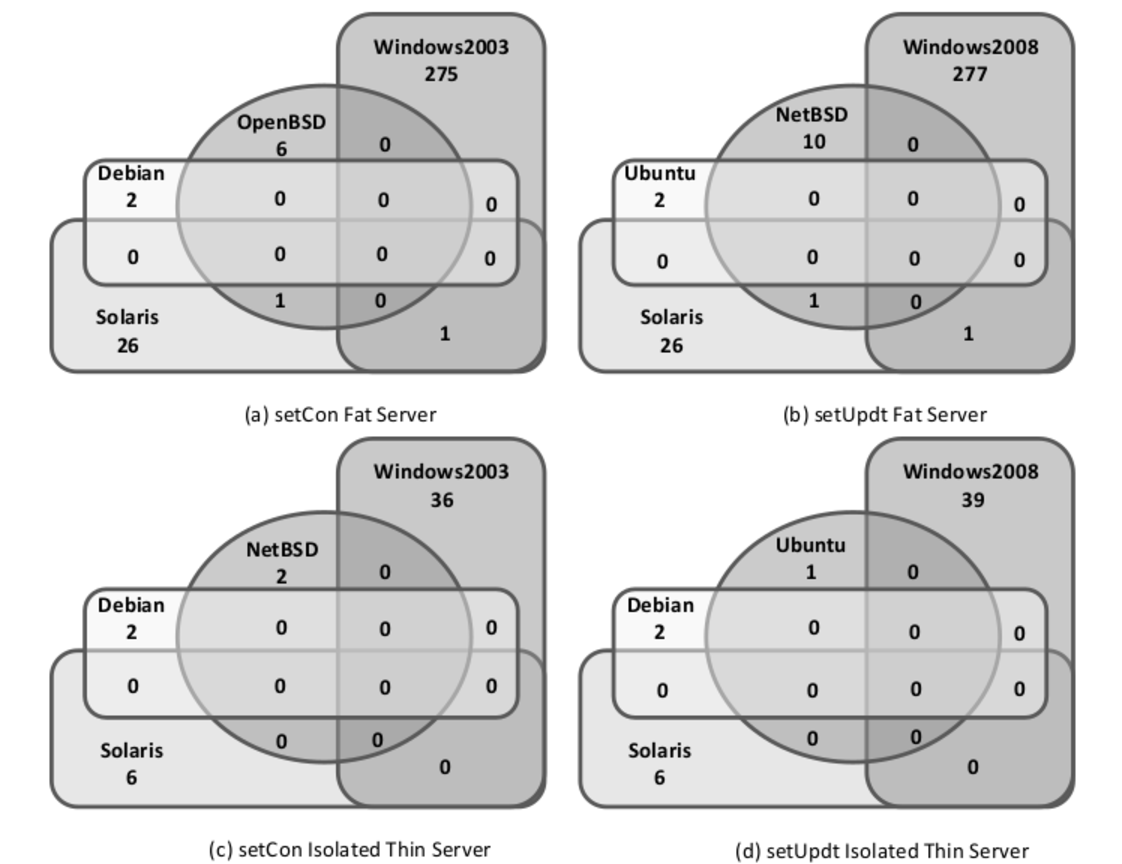
\includegraphics[scale=0.7]{images/images/grayscale_ven_dia_one_fig_update_a.pdf}
 \caption{Venn diagrams for vulnerabilities in setCon and setUpdt for strategies CVCst in Fat Server and Isolated Thin Server configurations.}
 \label{fig-venn_a}
\end{figure}


\subsubsection*{Common Vulnerability Indicator Strategy (CVIst)} 
This strategy employs the \gls{cvi} value, defined at the beginning of this section, to make decisions about including/excluding particular \glspl{os}.
Therefore, besides taking advantage of the available data on total counts of shared vulnerabilities, it also uses the information on how these numbers have evolved through the years.

\gls{cvis} is applied by executing the following method, which is based on minimizing a cost function. 
For a given year and time span, the \gls{cvi} value is calculated for each of the \gls{os} pairs. 
Typically, one should use the most recent year for which there is available data. 
The time span should cover a reasonable interval so that the indicator reflects the trend of discovered vulnerabilities. 
In some cases, however, one may have to resort to smaller time spans due to lack of data, namely with \glspl{os} released recently. 
In this case, the indicator will give a higher weight to the vulnerabilities reported in the last year. 
In \gls{cvis} the cost of creating a group with two \glspl{os} A and B is $\mathit{CVI}(A,B)$. 
Extending this idea to a group of $n$ \glspl{os}, the total cost becomes the sum of the individual \gls{cvi} for all combinations of \gls{os} pairs.
In order to choose the best groups, the strategy searches for sets of \glspl{os} that together have the smallest total cost.


\begin{table}[!ht]
\begin{center}
{\footnotesize
\begin{tabular}{|l|c|c|c|c|c|c|c|c|c|c|c|c|}\cline{2-11}
 \multicolumn{1}{c|}{} &
\begin{sideways}\vspace{2mm}\parbox{2mm}OpenBSD\end{sideways}&
\begin{sideways}\vspace{2mm}\parbox{2mm}NetBSD\end{sideways}&
\begin{sideways}\vspace{2mm}\parbox{2mm}FreeBSD\end{sideways}&
\begin{sideways}\vspace{2mm}\parbox{2mm}Solaris  \end{sideways}&
\begin{sideways}\vspace{2mm}\parbox{2mm}Debian\end{sideways}&
\begin{sideways}\vspace{2mm}\parbox{2mm}Ubuntu \end{sideways}&
\begin{sideways}\vspace{2mm}\parbox{2mm}RedHat\end{sideways}&
\begin{sideways}\vspace{2mm}\parbox{3mm}Win2000 \end{sideways}&
\begin{sideways}\vspace{2mm}\parbox{3mm}Win2003 \end{sideways}&
\begin{sideways}\vspace{2mm}\parbox{3mm}Win2008  \end{sideways}&
\multicolumn{2}{|c}{} \\ \cline{1-11}  \cline{1-12}
OpenBSD & - & 17.1 & 22.2 & 4.0 & 1.7 & 2.5 & 5.0 & 1.8 & 1.5 & 0.9 & \multirow{13}{1mm}{\begin{sideways}\hspace{8mm}\parbox{16mm}{$\mathit{CVI}_{2009}$(A,B)}\end{sideways}} \\ \cline{1-11}
NetBSD & 4 &  - & 19.7 & 4.9 & 1.4 & 0.0 & 1.8 & 1.6 & 1.5 & 0.9&\\ \cline{1-11}
FreeBSD & 4 & 6 & - & 6.5 & 1.3 & 1.3 & 5.6 & 2.3 & 2.0 & 0.9&\\ \cline{1-11}
Solaris & 1 & 1 & 2 & - & 1.0 & 1.5 & 5.3 & 5.5 & 5.6 & 0.0&\\ \cline{1-11}
Debian & 0 & 0 & 0 & 0 & - & 10.5 & 26.1 & 0.9 & 0.9 & 0.0&\\ \cline{1-11}
Ubuntu & 0 & 0 & 0 & 0 & 0 & - & 18.5 & 0.9 & 0.9 & 0.0&\\ \cline{1-11}
RedHat & 0 & 0 & 0 & 2 & 0 & 0 &  - & 1.4 & 1.8 & 0.0&\\ \cline{1-11}
Win2000 & 0 & 0 & 0 & 1 & 0 & 0 & 0 & - & 163.6 & 39.5&\\ \cline{1-11}
Win2003 & 0 & 0 & 0 & 1 & 0 & 0 & 0 & 49 & - & 0.0 &\\ \cline{1-12}
Win2008 & 0 & 0 & 0 & 1 & 0 & 0 & 0 & 38 & 229 & - &\multicolumn{1}{|c}{}  \\ \cline{1-11}
 \multicolumn{1}{c|}{}& \multicolumn{9}{|c|}{2010-2011} & \multicolumn{2}{|c}{}\\ \cline{2-10}
\end{tabular}
\caption{History/observed period for CVIst with Fat Servers.}
\label{tab:strat_ii}
}
\end{center}
\end{table}

To evaluate this strategy, we split the time into two intervals as we did for \gls{cvcs}. 
Table~\ref{tab:strat_ii} presents in the cells for the history period the $\mathit{CVI}_{2009}(A,B)$ for a time span of 10 years in a Fat Server configuration.\footnote{In some cases, we had to use smaller time spans due to the more recent release date of the \glspl{os} (e.g., Ubuntu and Windows 2008). When this happened, the \gls{cvi} value was calculated using the maximum time span that is allowed by the available data.}
The cells at left and bottom of the diagonal line correspond to the observed period, and they count as before the number of shared vulnerabilities in 2010 and 2011. After applying \gls{cvis}, the following sets are the best with four \glspl{os}:

\begin{itemize}
\item setCon = \{\emph{OpenBSD, Solaris, Debian, Windows2003}\}, with a total cost of $14.7$;
\item setUpdt = \{\emph{NetBSD, Solaris, Ubuntu, Windows2008}\}, with a total cost of $7.3$.
\end{itemize}

To verify if \gls{cvi} is a good indicator for selecting diverse sets, we can look at the number of common vulnerabilities in the observed period (2010--2011). 
By analyzing Table~\ref{tab:strat_ii}, it is possible to see that setCon and setUpdt remain good sets, each one with two shared flaws. 
As before with \gls{cvcs}, one can find better sets in observed period, where no common vulnerabilities appear for several pairs, for example by replacing Solaris with RedHat.
The Venn diagrams for these two sets are shown in Figures~\ref{fig-venn_b}(e) and~\ref{fig-venn_b}(f).

\begin{table}[!h]
\begin{center}
{\footnotesize
\begin{tabular}{|l|c|c|c|c|c|c|c|c|c|c|c|c|}\cline{2-11}
 \multicolumn{1}{c|}{} &
\begin{sideways}\vspace{2mm}\parbox{2mm}OpenBSD\end{sideways}&
\begin{sideways}\vspace{2mm}\parbox{2mm}NetBSD\end{sideways}&
\begin{sideways}\vspace{2mm}\parbox{2mm}FreeBSD\end{sideways}&
\begin{sideways}\vspace{2mm}\parbox{2mm}Solaris  \end{sideways}&
\begin{sideways}\vspace{2mm}\parbox{2mm}Debian\end{sideways}&
\begin{sideways}\vspace{2mm}\parbox{2mm}Ubuntu \end{sideways}&
\begin{sideways}\vspace{2mm}\parbox{2mm}RedHat\end{sideways}&
\begin{sideways}\vspace{2mm}\parbox{3mm}Win2000 \end{sideways}&
\begin{sideways}\vspace{2mm}\parbox{3mm}Win2003 \end{sideways}&
\begin{sideways}\vspace{2mm}\parbox{3mm}Win2008  \end{sideways}&
\multicolumn{2}{|c}{} \\ \cline{1-11}  \cline{1-12}
OpenBSD & - & 8.4 & 14.1 & 1.8 & 0.0 & 0.0 & 1.6 & 1.8 & 1.8 & 0.9  & \multirow{13}{1mm}{\begin{sideways}\hspace{8mm}\parbox{16mm}{$\mathit{CVI}_{2009}$(A,B)}\end{sideways}} \\ \cline{1-11}
NetBSD & 1 & - & 11.0 & 1.5 & 0.6 & 0.0 & 0.6 & 1.6 & 0.9 & 0.9&\\ \cline{1-11}
FreeBSD & 1 & 1 & - & 2.3 & 0.0 & 0.0 & 1.7 & 2.3 & 1.5 & 0.9&\\ \cline{1-11}
Solaris & 0 & 0 & 0 & - & 0.0 & 0.0 & 1.0 & 1.0 & 0.6 & 0.0&\\ \cline{1-11}
Debian & 0 & 0 & 0 & 0 & - & 1.9 & 3.2 & 0.9 & 0.9 & 0.0&\\ \cline{1-11}
Ubuntu & 0 & 0 & 0 & 0 & 0 &  - & 0.9 & 0.9 & 0.9 & 0.0&\\ \cline{1-11}
RedHat & 0 & 0 & 0 & 0 & 0 & 0 &- & 0.9 & 0.9 & 0.0&\\ \cline{1-11}
Win2000 & 0 & 0 & 0 & 0 & 0 & 0 & 0 & - & 58.7 & 12.5&\\ \cline{1-11}
Win2003 & 0 & 0 & 0 & 0 & 0 & 0 & 0 & 4 & - & 13.5&\\ \cline{1-12}
Win2008 & 0 & 0 & 0 & 0 & 0 & 0 & 0 & 3 & 26 & -&\multicolumn{1}{|c}{}  \\ \cline{1-11}
 \multicolumn{1}{c|}{}& \multicolumn{9}{|c|}{2010-2011} & \multicolumn{2}{|c}{}\\ \cline{2-10}
\end{tabular}
\caption{History/observed period for CVIst with Isolated Thin Servers.}
\label{tab:strat_ii_iso}
}
\end{center}
\end{table}


Table \ref{tab:strat_ii_iso} provides the data for applying CVIst in Isolated Thin Server configurations. 
It is possible to observe that \gls{cvi} values have significantly decreased when compared to the previous table. 
The best groups of four \glspl{os} in the historical period are:

\begin{itemize}
\item setCon = \{\emph{NetBSD, Solaris, Debian, Windows2003}\}, with a total cost of $4.5$;
\item setUpdt = \{\emph{Solaris, Debian, Ubuntu, Windows2008}\}, with a total cost of $1.9$.
\end{itemize}

By checking the data for the observed period, one can see that both sets do not share a single vulnerability, which indicates that the strategy would have made a good selection of \glspl{os} (see also the Venn diagrams in Figures~\ref{fig-venn_b}(g) and~\ref{fig-venn_b}(h)).


\begin{figure}[!h]
 \centering
 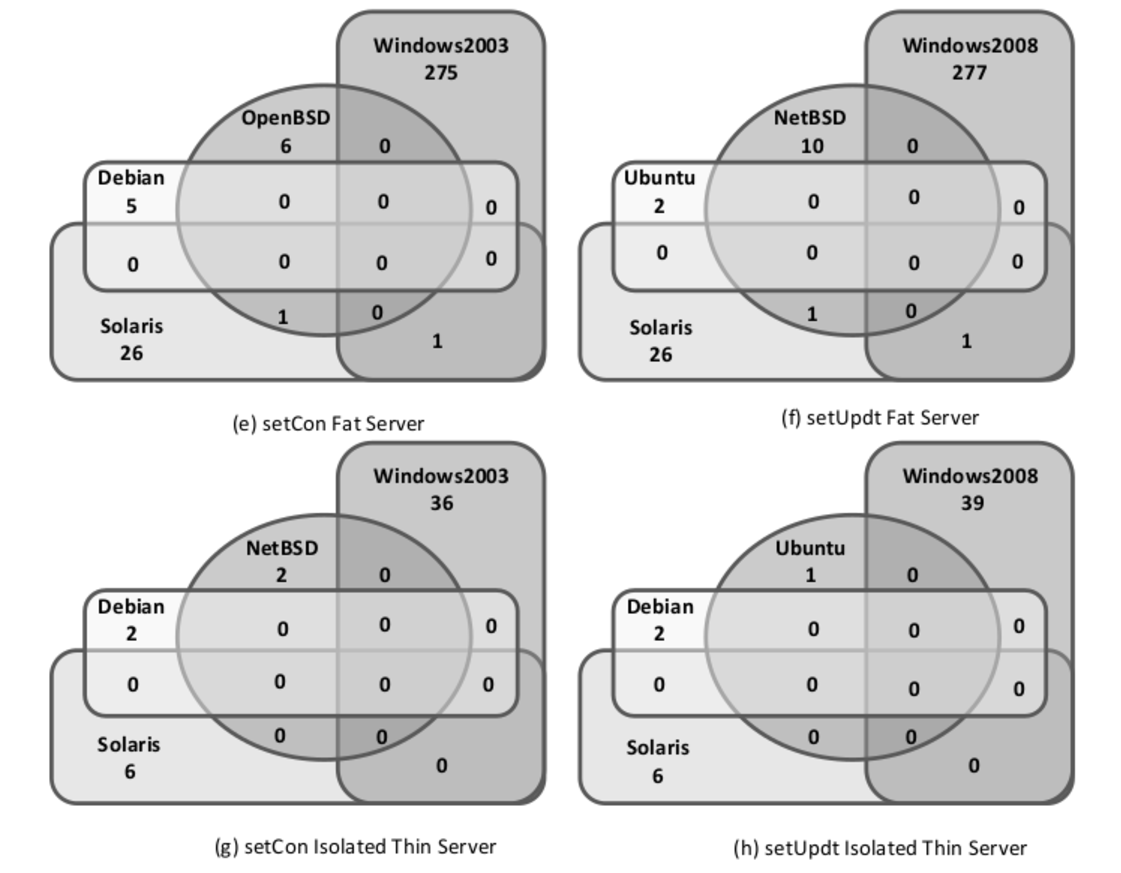
\includegraphics[scale=0.7]{images/images/grayscale_ven_dia_one_fig_update_b.pdf}
 \caption{Venn diagrams for vulnerabilities in setCon and setUpdt for strategies CVIst in Fat Server and Isolated Thin Server configurations.}
 \label{fig-venn_b}
\end{figure}

\subsubsection*{Inter-Reporting Times Strategy (IRTst)} \label{IRT} 
This strategy is mainly concerned with the \emph{\gls{irt}}, i.e., the number of days between successive reports of common vulnerabilities in different \gls{os} pairs, rather than vulnerability counts. 
The assumption underlying this strategy is that lower inter-reporting times suggest a greater similarity between \glspl{os}, and thus it would be advisable, from a diversity standpoint, to select \glspl{os} with higher \gls{irt}.

Table \ref{tab:pairs_irt} presents the number of vulnerabilities for each pair of \glspl{os} in five \gls{irt} intervals, from 0 to 10000 days.
The values in the table were obtained in the following manner: first, for a given \gls{os} pair A and B, we collected the dates for common vulnerabilities; next, we calculated the \gls{irt} in days of every two consecutive vulnerabilities; and then, we counted the number of vulnerabilities that were within each interval.
The table is organized such that on the top are the \glspl{os} without common vulnerabilities, which are then followed by the ones that had larger \gls{irt} values. 
Therefore, each horizontal line separates groups of \gls{os} pairs that have positive \gls{irt} values in the same leftmost column, starting from the rightmost column (i.e., with the longer \gls{irt}). 
From a diversity perspective, it is interesting to notice that in the table there are $29\%$ of the pairs that do not have two consecutive vulnerabilities, and that $11\%$ only have consecutive vulnerabilities from $1000$ days on (last column).


%TABLE VII

\begin{table}[!h]
\begin{center}
{\scriptsize
\begin{tabular}{|l||c c c c c|}\hline
&	0 $\leq$ IRT $\leq 1$	&	$1$ \textless IRT $\leq 10$	&	$10$ \textless IRT $\leq100$	&	$100$ \textless IRT $\leq 1000$	& $1000$ \textless IRT $\leq10000$\\\hline
OpenBSD-Win2008 & 0 & 0 & 0 & 0 & 0 \\
NetBSD-Ubuntu & 0 & 0 & 0 & 0 & 0 \\
NetBSD-Win2003 & 0 & 0 & 0 & 0 & 0 \\
NetBSD-Win2008 & 0 & 0 & 0 & 0 & 0 \\
FreeBSD-Win2008 & 0 & 0 & 0 & 0 & 0 \\
Solaris-Win2008 & 0 & 0 & 0 & 0 & 0 \\
Debian-Win2000 & 0 & 0 & 0 & 0 & 0 \\
Debian-Win2003 & 0 & 0 & 0 & 0 & 0 \\
Debian-Win2008 & 0 & 0 & 0 & 0 & 0 \\
Ubuntu-Win2000 & 0 & 0 & 0 & 0 & 0 \\
Ubuntu-Win2003 & 0 & 0 & 0 & 0 & 0 \\
Ubuntu-Win2008 & 0 & 0 & 0 & 0 & 0 \\
RedHat-Win2008 & 0 & 0 & 0 & 0 & 0 \\ \hline
OpenBSD-Win2003 & 0 & 0 & 0 & 0 & 1 \\
FreeBSD-Win2003 & 0 & 0 & 0 & 0 & 1 \\
Solaris-Debian & 0 & 0 & 0 & 0 & 1 \\
RedHat-Win2000 & 0 & 0 & 0 & 0 & 1 \\
OpenBSD-Win2000 & 0 & 0 & 0 & 0 & 2 \\ \hline
OpenBSD-Debian & 0 & 0 & 0 & 1 & 0 \\
Solaris-Ubuntu & 0 & 0 & 0 & 1 & 0 \\
NetBSD-Win2000 & 0 & 0 & 0 & 1 & 1 \\
FreeBSD-Win2000 & 0 & 0 & 0 & 2 & 1 \\ \hline
FreeBSD-Ubuntu & 0 & 0 & 1 & 0 & 0 \\
RedHat-Win2003 & 0 & 0 & 1 & 0 & 0 \\
OpenBSD-Solaris & 0 & 0 & 3 & 4 & 2 \\
FreeBSD-Solaris & 0 & 0 & 5 & 8 & 0 \\ \hline
FreeBSD-Debian & 0 & 1 & 0 & 2 & 0 \\ \hline
OpenBSD-Ubuntu & 1 & 0 & 0 & 1 & 0  \\
NetBSD-Debian & 1 & 0 & 0 & 1 & 0 \\
NetBSD-Solaris & 1 & 0 & 3 & 4 & 1 \\
Solaris-Win2003 & 1 & 1 & 1 & 4 & 0 \\
Solaris-Win2000 & 1 & 1 & 1 & 4 & 1 \\
NetBSD-RedHat & 2 & 0 & 0 & 3 & 0 \\
Solaris-RedHat & 2 & 0 & 0 & 7 & 0\\
FreeBSD-RedHat & 2 & 1 & 2 & 5 & 1\\
Debian-Ubuntu & 3 & 2 & 3 & 5 & 0\\
OpenBSD-RedHat & 4 & 0 & 1 & 4 & 0\\
NetBSD-FreeBSD & 4 & 3 & 20 & 14 & 0 \\
OpenBSD-NetBSD & 7 & 3 & 14 & 12 & 0 \\
Ubuntu-RedHat & 11 & 2 & 7 & 6 & 0 \\
OpenBSD-FreeBSD & 11 & 5 & 16 & 14 & 0 \\
Debian-RedHat & 22 & 3 & 18 & 8 & 0 \\
Win2000-Win2008 & 54 & 7 & 15 & 3 & 0 \\
Win2000-Win2003 & 167 & 29 & 66 & 2 & 0 \\
Win2003-Win2008 & 222 & 16 & 41 & 2 & 0 \\ \hline
\end{tabular}
\caption{Number of two consecutive vulnerabilities occurring in each \gls{irt} period, between 2000 and 2011 (with Fat Servers).}
\label{tab:pairs_irt}
}
\end{center}
\end{table}


The \gls{irts} strategy allows the selection of \glspl{os} with longer \gls{irt}. 
This criteria is essential if one wants to deploy a system that has a short lifetime, e.g., a batching process, which ideally would only be in operation between the discovery of common vulnerabilities. 
\gls{irts} tries first to select \gls{os} pair with zero common vulnerabilities; when this is not possible, it chooses the next pair whose common vulnerabilities appear in the rightmost columns. 
By inspecting the table, we can see that the best two sets of four \glspl{os} are:

\begin{itemize}
\item setCon = \{\emph{OpenBSD, Solaris, Debian, Windows2003}\};
\item setUpdt = \{\emph{NetBSD, Solaris, Ubuntu, Windows2008}\}.
\end{itemize}


Table \ref{tab:pairs_irt_iso} presents the \gls{irt} for an Isolated Thin Server configuration. 
Since each \gls{os} pair has less common vulnerabilities, this often translates to larger \gls{irt}.  
The percentage of lines with zero \gls{irt} in all intervals is higher, $51\%$, but remained the same for the \gls{os} pairs that share vulnerabilities with longer \gls{irt} ($11\%$). 
When applying the strategy to this table, the best sets of \glspl{os} are: 

\begin{itemize}
\item setCon = \{\emph{OpenBSD, Solaris, Debian, Windows2003}\};
\item setUpdt = \{\emph{OpenBSD, Debian, Ubuntu, Windows2008}\}.
\end{itemize}


\begin{table}[!ht]
\begin{center}
{\scriptsize
\begin{tabular}{|l||c c c c c|}\hline
&	$0$ $\leq$ IRT $\leq 1$	& $1$ \textless IRT $\leq 10$ & $10$ \textless IRT $\leq 100$ & $100$ \textless IRT $\leq 1000$ & $1000$ \textless IRT $\leq 10000$\\\hline
OpenBSD-Debian & 0 & 0 & 0 & 0 & 0 \\
OpenBSD-Ubuntu & 0 & 0 & 0 & 0 & 0 \\
OpenBSD-Win2008 & 0 & 0 & 0 & 0 & 0 \\
NetBSD-Ubuntu & 0 & 0 & 0 & 0 & 0 \\
NetBSD-Win2003 & 0 & 0 & 0 & 0 & 0 \\
NetBSD-Win2008 & 0 & 0 & 0 & 0 & 0 \\
FreeBSD-Debian & 0 & 0 & 0 & 0 & 0 \\
FreeBSD-Ubuntu & 0 & 0 & 0 & 0 & 0 \\
FreeBSD-Win2008 & 0 & 0 & 0 & 0 & 0 \\
Solaris-Debian & 0 & 0 & 0 & 0 & 0 \\
Solaris-Ubuntu & 0 & 0 & 0 & 0 & 0 \\
Solaris-Win2003 & 0 & 0 & 0 & 0 & 0 \\
Solaris-Win2008 & 0 & 0 & 0 & 0 & 0 \\
Debian-Win2000 & 0 & 0 & 0 & 0 & 0 \\
Debian-Win2003 & 0 & 0 & 0 & 0 & 0 \\
Debian-Win2008 & 0 & 0 & 0 & 0 & 0 \\
Ubuntu-RedHat & 0 & 0 & 0 & 0 & 0 \\
Ubuntu-Win2000 & 0 & 0 & 0 & 0 & 0 \\
Ubuntu-Win2003 & 0 & 0 & 0 & 0 & 0 \\
Ubuntu-Win2008 & 0 & 0 & 0 & 0 & 0 \\
RedHat-Win2000 & 0 & 0 & 0 & 0 & 0 \\
RedHat-Win2003 & 0 & 0 & 0 & 0 & 0  \\
RedHat-Win2008 & 0 & 0 & 0 & 0 & 0 \\ \hline
OpenBSD-Win2003 & 0 & 0 & 0 & 0 & 1 \\
FreeBSD-Win2003 & 0 & 0 & 0 & 0 & 1 \\
Solaris-RedHat & 0 & 0 & 0 & 0 & 1 \\
Solaris-Win2000 & 0 & 0 & 0 & 0 & 1  \\
OpenBSD-Win2000 & 0 & 0 & 0 & 0 & 2 \\ \hline
Debian-Ubuntu & 0 & 0 & 0 & 1 & 0 \\
NetBSD-Win2000 & 0 & 0 & 0 & 1 & 1 \\
FreeBSD-Win2000 & 0 & 0 & 0 & 2 & 1 \\ \hline
NetBSD-Solaris & 0 & 0 & 1 & 2 & 0 \\
OpenBSD-Solaris & 0 & 0 & 1 & 3 & 0 \\
FreeBSD-Solaris & 0 & 0 & 1 & 4 & 0 \\ \hline
NetBSD-Debian & 1 & 0 & 0 & 0 & 0  \\
NetBSD-RedHat & 1 & 0 & 0 & 0 & 0 \\
Debian-RedHat & 1 & 0 & 1 & 3 & 2 \\
OpenBSD-RedHat & 2 & 0 & 0 & 0 & 0 \\
FreeBSD-RedHat & 2 & 0 & 0 & 0 & 0 \\
OpenBSD-NetBSD & 2 & 0 & 3 & 7 & 1 \\
NetBSD-FreeBSD & 2 & 0 & 6 & 9 & 1 \\
OpenBSD-FreeBSD & 6 & 0 & 9 & 10 &  1\\
Win2000-Win2008 & 8 & 1 & 3 & 3 & 0 \\
Win2003-Win2008 & 16 & 2 & 19 & 2 & 0 \\
Win2000-Win2003 & 35 & 8 & 36 & 5 & 0\\ \hline
\end{tabular}
\caption{Number of two consecutive vulnerabilities occurring in each IRT period, between 2000 and 2011 (Isolated Thin Servers).}
\label{tab:pairs_irt_iso}
}
\end{center}
\end{table}

\subsubsection*{Comparing the three strategies}
In one hand, the three strategies explore distinct characteristics of the data to pick the \glspl{os} to be deployed. 
Qualitatively they differ in the method of selection, and potentially the result of applying them to our data could lead to distinct sets being chosen.
On the other hand, all of them try to find \glspl{os} that when placed together in the same system have a low probability of experiencing common vulnerabilities in the future. 
Therefore, if there is a small collection of \gls{os} sets with this property, then all strategies should elect one of these sets as the best choice. 
This is precisely what we observed with the \gls{nvd} data, and consequently, the selected best sets are not too different from each other.
Only when one needs to find many \gls{os} sets with reasonable levels of diversity, such as with the implementation of proactive recovery mechanisms in intrusion-tolerant systems~\cite{Castro:2002,Sousa:2010}, then the distinctions among the strategies start to become apparent.
We leave it as future work a more refined study on the comparison of the strategies with larger groups of \gls{os} sets.

The \gls{os} sets that resulted from the execution of the strategies achieved reasonable levels of diversity when evaluated in the observed period (years 2010 and 2011). 
As expected from our analysis, several of the best sets contained an \gls{os} from each of the families. 
The exception to this rule occurred with the Linux family, wherein a few cases it had two representatives (Debian and Ubuntu) because these \glspl{os} had very few vulnerabilities reported in the last three years. 
Even though the BSD family also had a small number of recent vulnerabilities, since these occasionally affected more \glspl{os}, the strategies opted for including just one of the BSD \glspl{os}.

In the next section, we will look into \gls{os} versions as a way to increase diversity. 
For this study, we will use the set that was most selected by the different strategies: \{\emph{OpenBSD, Debian, Solaris, Windows2003}\} (4 out of 12 choices, considering both Fat Server and Isolated Thin Server configurations).


%%%%%%%%%%%%%%%%%%%%%%%%%%%%%%%%%%%%%%%%%%%%%%%%%%%%%%%%%%%%%%%%%%%%%%%%%%%%%%%%%%%%%%%%%%%
\subsection{Exploring Diversity Across OS Releases}
\label{releases}

If one wants to build systems capable of tolerating a few intrusions, our results show that it is possible to select \glspl{os} for the replicas with a small collection of common vulnerabilities. 
It is hard, however, to support critical services that need to remain correct with higher numbers of compromised replicas or to use some \gls{bft} algorithms that trade off performance for extra replicas (e.g., \cite{Abd-El-Malek:2005,Kotla:2010,Serafini:2010}). 
The number of available \glspl{os} is limited, and consequently, one rapidly runs out of different \glspl{os} (e.g., 13 distinct \glspl{os} are needed to tolerate $f=4$ faults in a $3f+1$ system). 
However, our experiments are relatively pessimistic in the sense that they are based on long periods of time, and no distinctions are made between \gls{os} releases.

Newer releases of an \gls{os} can contain essential code changes, and therefore, old vulnerabilities may disappear and/or new vulnerabilities may be introduced. 
As a result, if we consider (OS, release) pairs, one may augment the number of different systems that do not share vulnerabilities. 
%Nevertheless, one should keep in mind that the use of older \gls{os} releases does not come without a cost. Namely, there might be incompatibilities with the current hardware, and some older software packages might be challenging to find.

%In the next two sections we explore \emph{n-diverse} sets, where we extend the OS, as an element in the set, to the \gls{os} release. 

%First we study a \emph{4-diverse} set, and then a \emph{2-diverse} set built with only two \glspl{os}. 
%We will concentrate on Isolated Thin Server configurations because they correspond to the most common way to deploy intrusion-tolerant systems.


\subsubsection*{Sets with Four Diverse OSes}
In this section, we explore the diversity of a particular \emph{4-diverse} set in the Isolated Thin Server configuration.
In particular, we analyze in more detail the vulnerabilities for the set \{\emph{OpenBSD, Debian, Solaris, Windows2003}\} across their releases between 2000 and 2011. 
Despite the year of the release, since some vulnerabilities can be inherited from older versions of the code, we will include all vulnerabilities no matter the published date (i.e., even the flaws before 2000).

From all releases available for our 4-version replicated system,\footnote[1]{OpenBSD~2.7, OpenBSD~2.8, OpenBSD~2.9, OpenBSD~3.0, OpenBSD~3.1, OpenBSD~3.2, OpenBSD~3.3, OpenBSD~3.4, OpenBSD~3.5, OpenBSD~3.6, OpenBSD~3.7, OpenBSD~3.8 OpenBSD~3.9, OpenBSD~4.0, OpenBSD~4.1, OpenBSD~4.2, OpenBSD~4.3, OpenBSD~4.4,   Solaris~10.0, Solaris~11.0, Solaris~8.0, Solaris~8.1, Solaris~8.2, Solaris~9.0, Solaris~9.1, Debian~2.2, Debian~2.3, Debian~3.0,   Debian~3.1, Debian~4.0, Debian~6.0, Debian~6.2, and Windows~2003.} we looked at the major releases that had non-zero vulnerabilities. 
Since OpenBSD follows a fixed six-month release cycle, in this case, we selected one version every three years, which is reasonable given our 12-year time span (considering all 18 releases would require 154 entries in the table). 
Therefore, the \gls{os} releases that are taken into the study are: OpenBSD 5.0, OpenBSD 4.4, OpenBSD 3.8, OpenBSD 3.2, Solaris 8.0, Solaris 9.0, Solaris 10.0, Solaris 11.0, Debian 2.2, Debian 3.0, Debian 4.0, Debian 5.0, Debian 6.0 and Windows2003.

\begin{table}[!ht]
\begin{center}
{\scriptsize
\begin{tabular}{|l|c|}\hline
\textbf{OS Versions} & Total  \\\hline\hline
Solaris 8.0-Solaris 9.0 	&21\\
Solaris 9.0-Solaris 10.0 	&8\\
Solaris 8.0-Solaris 10.0 	&7\\
OpenBSD 3.2-OpenBSD 3.8 & 4 \\
OpenBSD 3.2-Solaris 9.0 & 2 \\
OpenBSD 3.2-Windows2003 & 2 \\
OpenBSD 3.2-Solaris 8.0 & 1 \\
OpenBSD 3.8-Windows2003 & 1 \\
Solaris 8.0-Windows2003 & 1 \\
Solaris 9.0-Windows2003 & 1 \\
Solaris 10.0-Windows2003 & 1 \\
Solaris 10.0-Solaris 11.0	& 1 \\
Solaris 8.0-Debian 2.2 &	1 \\
Debian 4.0-Windows2003 & 1 \\\hline
\end{tabular}
\caption{Common vulnerabilities between OS releases.}
\label{tab:vulns_releases}
}
\end{center}
\end{table}

Table \ref{tab:vulns_releases} shows the number of common vulnerabilities for each pair of OS-release (pairs with zero values are not displayed). 
The first observation is that there are many releases within this set of 4 \glspl{os} that appear to be free of common flaws. 
Second, these shared bugs occur more often between releases of the same \gls{os}. 
This is anticipated because more code is re-used within the same \gls{os}.
Additionally, one can notice that releases of the same \gls{os} typically have less shared vulnerabilities when comparing older and newer versions. 
This is particularly evident for the OpenBSD and Debian releases. 
This result is quite promising because it supports our thesis that one should be able to explore diversity across releases, as a way to increase the number of available candidates for the construction of the diverse \gls{os} sets.


%\subsubsection*{2-diverse sets} 
%To reduce the development and maintenance costs of an intrusion-tolerant system, it is reasonable to investigate solutions that attempt to decrease the number of distinct \glspl{os} but still ensure %a high level of security. 
%Here, it makes sense to consider an approach that offers diversity with only two \glspl{os}, while still exploiting the diversity available within the \gls{os} releases. 
%In the extreme case, one can select \glspl{os} from the same family, for instance, to simplify system management.

%To study this sort of solution, we looked at the vulnerabilities that appeared in several versions of Debian and RedHat (all released after 2000). 
%In total, seven Debian and ten RedHat releases were considered, which gives a total of $136$ combinations. 
%Table \ref{tab:debian_RedHat} provides a summary of the vulnerabilities that were found in \gls{nvd} for pairs of \gls{os} releases (to save space, we omit pairs with zero common vulnerabilities). 
%The reader should notice that RedHat went through two distinct distributions from 2000, and they can be distinguished by the version number: RedHat Linux existed between 2000 and 2003, and it has %a dot in the version number (e.g., RedHat 7.1); RedHat Enterprise Linux is available from 2003, and its releases only have a single digit (e.g., RedHat 3).

%\begin{table}[!ht]
%\begin{center}
%{\scriptsize
%\begin{tabular}{|l|c||l|c|}\hline
%\textbf{OS Versions} & Total &  \textbf{OS Versions} & Total \\\hline\hline
%Debian 2.2 - Debian 2.3 & 2 & RedHat 7.1 - RedHat 9.0 & 2  \\\hline
%Debian 3.1 - Debian 4.0 & 1 & RedHat 7.2 - RedHat 7.3 & 5  \\\hline
%Debian 4.0 - RedHat 3 & 1 &  RedHat 7.2 - RedHat 8.0 & 5  \\\hline
%Debian 4.0 - RedHat 4 & 1 & RedHat 7.2 - RedHat 9.0 & 2  \\\hline
%Debian 4.0 - RedHat 5 & 1 & RedHat 7.3 - RedHat 8.0 & 5  \\\hline
%RedHat 7.0 - RedHat 7.1 & 2 & RedHat 7.3 - RedHat 9.0 & 2  \\\hline
%RedHat 7.0 - RedHat 7.2 & 1 & RedHat 8.0 - RedHat 9.0 & 2  \\\hline
%RedHat 7.1 - RedHat 7.2 & 3 &  RedHat 3 - RedHat 4 & 2  \\\hline
%RedHat 7.1 - RedHat 7.3 & 2 & RedHat 3 - RedHat 5 & 1  \\\hline
%RedHat 7.1 - RedHat 8.0 & 2 &  RedHat 4 - RedHat 5 & 1  \\\hline
%\end{tabular}
%\caption{Common vulnerabilities between Debian and RedHat releases.}
%\label{tab:debian_RedHat}
%}
%\end{center}
%\end{table}

%The table only shows $14.7\%$ of the \gls{os} releases combinations, which means $85.3\%$ of the \gls{os} pairs are free from common flaws. 
%Debian has very few vulnerabilities that are shared between versions. 
%Moreover, accordingly to \gls{nvd}, these few vulnerabilities only affect two releases, i.e., no vulnerability had an impact over an extensive period. 
%There are two vulnerabilities, CVE-2003-0248 and CVE-2003-0364, that appear in five RedHat releases (from RedHat 7.1 to RedHat 9.0). 
%The first is a vulnerability in the \emph{mxcsr} kernel code which lets attackers modify CPU state registers via a malformed address. 
%This is a critical vulnerability because it has an impact on availability, confidentiality, and integrity. 
%The second one is in the RedHat TCP/IP implementation, and allows a \gls{dos} by CPU consumption. 
%Three vulnerabilities occur in RedHat 7.2, 7.3 and 8.0, all related to particular versions and configurations of the OpenSSL cryptographic toolkit. 
%When exploited, they cause a \gls{dos} (CVE-2004-0079, CVE-2004-0081 and CVE-2004-0112).
%Again, we can observe that few high impact vulnerabilities cross many versions of the same \gls{os}. 

%These results demonstrate that with a careful selection of the Debian and RedHat releases, it is possible to avoid most of the common vulnerabilities, and apparently, it becomes viable to build an intrusion-tolerant replicated system based on only two \glspl{os}.


\section{Decisions About Deploying Diversity}\label{decisions}
We have underscored that these results are only \textit{prima facie} evidence for the usefulness of diversity. 
On average, we would expect our estimates to be conservative as we analyzed aggregated vulnerabilities across releases: common vulnerabilities could be much smaller in a ``specific set'' of diverse \gls{os} releases. 
However, there are limitations on what can be claimed from the analysis of the \gls{nvd} data alone without further manual analysis (other than what we have done, e.g., developing/finding and running exploit scripts on every \gls{os} for each vulnerability).
A better analysis would be obtained if the \gls{nvd} vulnerability reports were combined with the exploit reports (including exploiting counts), and even better if they also had indications about the users' usage profile.
Moreover, we have seen that \gls{nvd} has some limitations, as we have found that some of the vulnerabilities were not reported in the \gls{nvd}, but several security advisory websites have reported those vulnerabilities.
Additionally, there are partial exploit reports available from other sites (e.g., \cite{cvedetails}).


Given these limitations, \emph{how can individual user organizations decide whether diversity is a suitable option for them, with their specific requirements and usage profiles?}
The cost is reasonably easy to assess: costs of the software products, the required middleware (if any), added the complexity of management, difficulties with client applications that require vendor-specific features, hardware costs, run-time cost of the synchronization and consistency enforcing mechanisms, and possibly more complex recovery after some failures.
The gains in improved security (from some tolerance to zero-day vulnerabilities and easier recovery from some exploits, set against possible extra vulnerabilities due to the increased complexity of the system) are difficult to predict except empirically. 


The first step onto adopting diversity as a dependable mechanism is done. 
The other limitations will be addressed in the rest of this thesis. 


\section{Final Remmarks}

In this chapter we presented results from an analysis of 18 years (1994--2011) of vulnerability reports from the \gls{nvd} database. 
It is worth to notice that the main manual work of analyzing the 2270 vulnerabilities of eleven \gls{os} distributions was done before this thesis. 
In this thesis, we developed three strategies to deploy diverse sets, some of which the ideas will be used in Chapter~\ref{chap:lazarus_design}.
In particular, the \gls{cvis}, as it introduces the notion of time evolution, which is fundamental for the following contributions.
In this first chapter of contributions, we intended to reinforce the answer to the main questions that drove our research for this thesis: 
\emph{what are the potential security gains that could be attained from using diverse \glspl{os} in a replicated intrusion-tolerant system?}
 
